\begin{flushright} {\tiny {\color{gray} basis\_q1fortin\_2D.tex}} \end{flushright}
%~~~~~~~~~~~~~~~~~~~~~~~~~~~~~~~~~~~~~~~~~~~~~~~~~~~~~~~~~~~~~~~~~~~~~~~~~~~~~~~~~~~~~~~~~~~~~~~~~~

We here consider the enriched $Q_1\times P_0$ element introduced first by 
Fortin (1981) \cite{fort81}.
The layout of the degrees of freedom is as follows:

\begin{flushright} {\tiny {\color{gray} (tikz\_q1pp02D.tex)}} \end{flushright}
%~~~~~~~~~~~~~~~~~~~~~~~~~~~~~~~~~~~~~~~~~~~~~~~~~~~~~~~~~~~~~~~~~~~~~~~~~~~~~~~~~~~~~~~~~~~~~~~~~~

\begin{center}
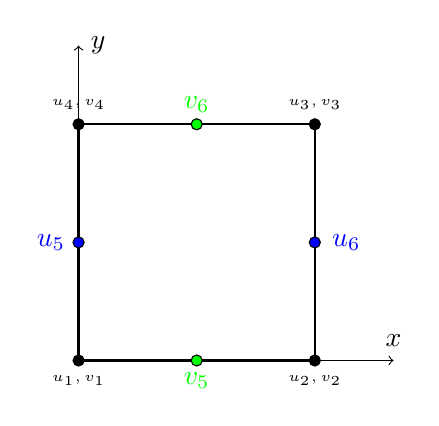
\begin{tikzpicture}
%\draw[fill=gray!23,gray!23](0,0) rectangle (6,5);
%\draw[step=0.5cm,gray,very thin] (0,0) grid (6,5); %background grid

\draw[thick] (1,.5) -- (4,.5) -- (4,3.5) -- (1,3.5) -- cycle; %front

\draw[thin,->] (4,0.5) -- (5,0.5); %x
\draw[thin,->] (1,3.5) -- (1,4.5); %y
\node[] at (5,0.75) {$x$};
\node[] at (1.25,4.5) {$y$};

\draw[black,fill=black] (1,.5)   circle (2pt);
\draw[black,fill=black] (4,.5)   circle (2pt);
\draw[black,fill=black] (4,3.5)   circle (2pt);
\draw[black,fill=black] (1,3.5)   circle (2pt);

\node[] at (1,0.25) {\tiny $u_1,v_1$};
\node[] at (4,0.25) {\tiny $u_2,v_2$};
\node[] at (4,3.75) {\tiny $u_3,v_3$};
\node[] at (1,3.75) {\tiny $u_4,v_4$};

\draw[black,fill=blue] (1,2) circle (2pt); 
\draw[black,fill=blue] (4,2) circle (2pt); 
\node[] at (0.65,2) {\color{blue} $u_5$};
\node[] at (4.4,2) {\color{blue} $u_{6}$};

\draw[black,fill=green] (2.5,0.5) circle (2pt); 
\draw[black,fill=green] (2.5,3.5) circle (2pt); 
\node[] at (2.5,0.25) {\color{green} $v_5$};
\node[] at (2.5,3.75) {\color{green} $v_{6}$};

\end{tikzpicture}\\
\end{center}


\noindent The approximation of the velocity components $u$ and $v$ inside the element is
\[
u^h(r,s) = a^u \; \bN_1(r,s) + b^u \;  \bN_2(r,s) + c^u \; \bN_3(r,s) +d^u \; \bN_4(r,s) 
+ d\; b_5^u(r,s) + e\; b_{6}^u(r,s)
\]
\[
v^h(r,s) = a^v \; \bN_1(r,s) + b^v \;  \bN_2(r,s) + c^v \; \bN_3(r,s) +d^v \; \bN_4(r,s) 
+ d^v b_5^v(r,s) + e^v b_{6}^v(r,s)
\]
where $\bN_{1,2,3,4}$ are the standard $Q_1$ basis functions in 2D and with 
\[
b_5^u(r,s) = \frac{1}{2}(1-r)(1-s^2)
\qquad
b_6^u(r,s) = \frac{1}{2}(1+r)(1-s^2)
\]
and
\[
b_5^v(r,s) = \frac{1}{2}(1-r^2)(1-s)
\qquad
b_6^v(r,s) = \frac{1}{2}(1-r^2)(1+s)
\]
In the end one arrives at

\begin{mdframed}[backgroundcolor=blue!5]
\begin{eqnarray}
{\bN}_1^u(r,s) &=&  \bN_1(r,s) - \frac{1}{2} b_5^u(r,s)\nn\\
{\bN}_2^u(r,s) &=&  \bN_2(r,s) - \frac{1}{2} b_6^u(r,s)\nn\\
{\bN}_3^u(r,s) &=&  \bN_3(r,s) - \frac{1}{2} b_6^u(r,s)\nn\\
{\bN}_4^u(r,s) &=&  \bN_4(r,s) - \frac{1}{2} b_5^u(r,s)\nn\\
{\bN}_5^u(r,s) &=&  b_5^u(r,s) \nn\\
{\bN}_6^u(r,s) &=&  b_6^u(r,s) \nn\\
\nn\\
{\bN}_1^v(r,s) &=&  \bN_1(r,s) - \frac{1}{2} b_5^v(r,s)\nn\\
{\bN}_2^v(r,s) &=&  \bN_2(r,s) - \frac{1}{2} b_5^v(r,s)\nn\\
{\bN}_3^v(r,s) &=&  \bN_3(r,s) - \frac{1}{2} b_6^v(r,s)\nn\\
{\bN}_4^v(r,s) &=&  \bN_4(r,s) - \frac{1}{2} b_6^v(r,s)\nn\\
{\bN}_5^v(r,s) &=&  b_5^v(r,s) \nn\\
{\bN}_6^v(r,s) &=&  b_6^v(r,s) 
\end{eqnarray}
\end{mdframed}

We can check for the zero-th order consistency: Let $u(r,s)=C$, then 
\begin{eqnarray}
u^h(r,s) 
= \sum_{i=1}^6 \bN_i^u(r,s) u_i 
= C \sum_{i=1}^6 \bN_i^u(r,s) 
= C \sum_{i=1}^4 \bN_i(r,s)  
= C
\end{eqnarray}





